%% LaTeX Beamer presentation template (requires beamer package)
%% see http://latex-beamer.sourceforge.net/
%% idea contributed by H. Turgut Uyar
%% template based on a template by Till Tantau
%% this template is still evolving - it might differ in future releases!

\documentclass[14pt]{beamer}

%\mode<presentation>
\mode<handout>
{
\usetheme{Berlin}

\setbeamercovered{transparent}
}

\usepackage[english]{babel}
\usepackage[latin1]{inputenc}


% font definitions, try \usepackage{ae} instead of the following
% three lines if you don't like this look
%%%\usepackage{mathptmx}
%%%\usepackage[scaled=.90]{helvet}
%%%\usepackage{courier}

\ifx\pdftexversion\undefined
\usepackage[dvips]{graphicx}
\else
\usepackage{graphicx}
\DeclareGraphicsRule{*}{mps}{*}{}
\fi

\usepackage{graphics}
%\usepackage{makeidx}
%\usepackage{mathpazo}
%\usepackage{multicol}
%\usepackage{srcltx}
\usepackage{color}
\usepackage{eurosym}
\usepackage{tikz}
\usepackage{pgfplots}
\pgfplotsset{every axis plot/.append style={very thick}}


\title{ISDN - Handlungsschritt eins}

%\subtitle{}

% - Use the \inst{?} command only if the authors have different
%   affiliation.
%\author{F.~Author\inst{1} \and S.~Another\inst{2}}
\author{Petra~Fronius \and Conrad~Kostecki \and Oluf~Lorenzen \and Christoph~Ringe \and Martin~Wilke}
% \inst{}

% - Use the \inst command only if there are several affiliations.
% - Keep it simple, no one is interested in your street address.
\institute
{
\inst \normalfont
Multi Media\\
\normalfont
Berufsbildende Schulen\\
}

\date{LF 9\\15. 12. 2008}


% This is only inserted into the PDF information catalog. Can be left
% out.
%%%\subject{Talks}



% If you have a file called "university-logo-filename.xxx", where xxx
% is a graphic format that can be processed by latex or pdflatex,
% resp., then you can add a logo as follows:

\pgfdeclareimage[height=0.5cm]{mmbbslogo}{mmbbslogo}
 \logo{\pgfuseimage{mmbbslogo}}



% Delete this, if you do not want the table of contents to pop up at
% the beginning of each subsection:
%%\AtBeginSubsection[]
%{
%\begin{frame}<beamer>
%\frametitle{Vorgehensweise}
%\tableofcontents[currentsection,currentsubsection]
%\end{frame}
%}

% If you wish to uncover everything in a step-wise fashion, uncomment
% the following command:

%\beamerdefaultoverlayspecification{<+->}

\begin{document}

\begin{frame}
\titlepage
\end{frame}

\begin{frame}
\frametitle{Einleitung}
\footnotesize{\tableofcontents}
% You might wish to add the option [pausesections]
\end{frame}


\section{ISDN}
\subsection{Definition und Merkmale}
\begin{frame}
\begin{itemize}
\item Integrated Services Digital Network
\item Internationaler Standard f�r digitales Kommunikationsnetzwerk
\item Integration verschiedener Dienste z.B. Telefonie, Telefax, Daten�bertragung
\item Zwei Anschlussvarianten
\begin{itemize}
  \item Basisanschluss
  \item Anlagenanschluss
\end{itemize}
%  \item fictitious settings \& actions
%  \vskip0pt plus.3fill
%  \item scripted or based on spontaneous acting
%  \vskip0pt plus.3fill
%  \item being someone else than yourself
\end{itemize}
\end{frame}

\subsubsection*{Basisanschluss}
\begin{frame}
\frametitle{Basisanschluss}
\begin{itemize}
  \item Zwei Nutzkan�le (B-Kan�le) mit je 64 Kbit/s
  \begin{itemize}
    \item Telefonie, Telefax \ldots
  \end{itemize}
  \item Ein Steuerkanal (D-Kanal) mit 16 Kbit/s
  \begin{itemize}
    \item Steuerinformationen
  \end{itemize}
  \item Nutzung von Privatkunden und kleineren Betrieben
\end{itemize}
\end{frame}

\subsubsection*{Anlagenanschluss}
\begin{frame}
\frametitle{Anlagenanschluss}
\begin{itemize}
  \item Anschluss einer Telefonanlage
  \item Eine Grundrufnummer mit beliebiger Anzahl von Durchwahlen
  \item Nutzung von mittelst�ndischen bis gro�en Betrieben 
\end{itemize}
\end{frame}

\subsubsection*{Prim�rmultiplex-Anschluss}
\begin{frame}
\frametitle{Prim�rmultiplex-Anschluss}
\begin{itemize}
  \item Besondere Form des Anlagenanschlusses
  \item 30 B-Kan�le mit je 64 Kbit/s
  \item Ein D-Kanal mit 64 Kbit/s
  \item Ein Kanal f�r Synchronisation und Wartung mit 64 Kbit/s
\end{itemize}
\end{frame}

\subsection{Vergleich von ISDN- und Analog-Anschl�ssen}
\begin{frame}
\begin{small}
\begin{columns}[c]
\column{1.8in}
Analog-Anschl�sse:
	\begin{itemize}
      \item 1 Kanal
      \item 1 Rufnummer
      \item 56 Kbit/s
      \item Signalverst�rkung\\
      \item Basispreis: 17~\euro/Monat
    \end{itemize}
\column{1.8in}
ISDN-Anschl�sse:
	\begin{itemize}
      \item 2 Kan�le
      \item 1 - 10 Rufnummern
      \item 128 Kbit/s
      \item Signalregenerierung\\
      \item Basispreis: 17,90~\euro/Monat
    \end{itemize}
\end{columns}
\end{small}
\end{frame}

%\subsection{Kosten von ISDN- und Analog-Anschluss}
%\begin{frame}
%	\begin{figure}[htb]
%		\centering
%		\begin{tikzpicture}
%			\begin{axis}[
%				xlabel=Zeit (s),
%				ylabel=Kraft (N),
%				width=7cm,
%				height=3cm]
%			\addplot[smooth,color=blue] 
%				table[x=time,y=datadownsampled] {demo.table};
%			\end{axis}
%		\end{tikzpicture}
%	\end{figure}
%\end{frame}

\subsection{Merkmale einer ISDN-TK-Anlage}
\begin{frame}
	\begin{itemize}
      \item Punkt zu Mehrpunkt-Verbindung
      \item Eine Rufnummer mit beliebigen Durchwahlnummern
      \begin{itemize}
	      \item Rufumleitung
	      \item Weiterverbinden
	      \item zentrales Telefonbuch
	      \item Geb�hrenerfassung
	  \end{itemize}
      \item Kostenlose interne Gespr�che
      \item Konferenzschaltungen\\
      \item Aktueller Basispreis: 17,90 \euro/Monat 
    \end{itemize}
\end{frame}


\section{DSL}
\subsection{Definition und Merkmale}
\begin{frame}
\frametitle{DSL}
	\begin{itemize}
      \item Digital Subscriber Line
      \item �bertragungsstandard mit bis zu 200 MBit via Kupferkabel
      \item DSL ``standalone''
      \item DSL �ber POTS
      \item DSL �ber ISDN
    \end{itemize}
    % FREQUENZSPEKTRUM-BILD!
\end{frame}

\subsection{ADSL}
\begin{frame}
\frametitle{ADSL}
	\begin{itemize}
      \item Asymmetric Digital Subscriber Line
      \item Prim�r f�r Privatanwender
      \item Downstream h�her als Upstream
      \item ADSL
      \item ADSL2 \& ADSL2+
    \end{itemize}
    % T-DSL-Angebot
\end{frame}

\subsection{SDSL}
\begin{frame}
\frametitle{SDSL}
	\begin{itemize}
      \item Symmetric Digital Subscriber Line
      \item Prim�r f�r Businessanwender
      \item Downstream entspricht Upstream
      \item Kein Festnetzanschluss m�glich, deswegen als Datenanschluss bezeichnet
      \item Aktuell bis zu 20 MBit realisierbar
    \end{itemize}
\end{frame}


%\subsection{Vergleich der Transferdauer bei ADSL und SDSL}
%\begin{frame}
%\end{frame}

\subsection{Kosten eines DSL-Anschlusses}

\begin{frame}[plain]
\frameheading{Kosten eines DSL-Anschlusses - ADSL}
\begin{figure}
\begin{center}
  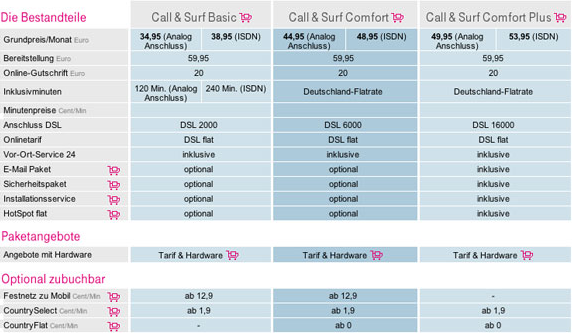
\includegraphics[width=1\textwidth]{DSL}
\end{center}
\end{figure}
\end{frame}

\begin{frame}[plain]
\frameheading{Kosten eines DSL-Anschlusses - SDSL}
\begin{figure}
\begin{center}
  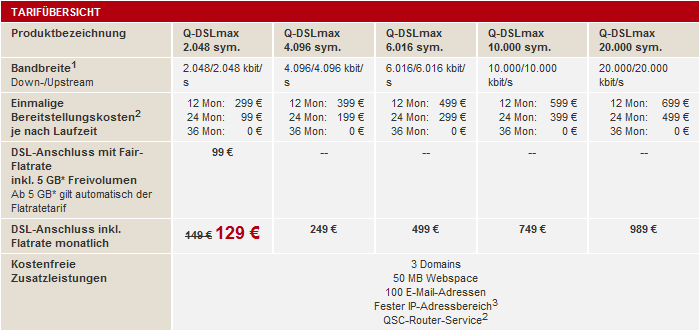
\includegraphics[width=1\textwidth]{SDSL}
\end{center}
\end{figure}
\end{frame}


\section{Allgemein}
\subsection{Transferdauer}

\begin{frame}
\frameheading{Transferdauer - Analog, ISDN, ISDN*2, ADSL}
\begin{footnotesize}
\begin{figure}
\begin{tikzpicture}
    \begin{axis}[
        xbar,
        xlabel=Dauer in Sekunden (10 Mb),
        width=3.5inch,
        height=2inch,
        ytick={1,...,4},
        yticklabels={%
            56 Kbps,
            64 Kbps,
            128 Kbps,
            8 Mbps},
        xmin=0,
        xmax=1600
    ]
    \addplot[draw=darkblue,fill=blue!50!white,semithick] coordinates {
        (1428,    1) 
        (1250,    2)
        (625,   3)
        (9,    4)
    };
    \end{axis}
\end{tikzpicture}
\end{figure}
%\end{columns}
\end{footnotesize}
\end{frame}

%\begin{small}
%\begin{columns}[c]
%\column{1.8in}
\begin{frame}
\frameheading{Transferdauer - ADSL \& SDSL}
\begin{footnotesize}
\begin{figure}
	\begin{tikzpicture}
	    \begin{axis}[
	        xbar,
	        xlabel=Dauer in Sekunden (10 Mb),
	        width=3.5inch,
	        height=2inch,
	        ytick={1,...,4},
	        yticklabels={%
	            Download ADSL,
	            Download SDSL,
	            Upload ADSL,
	            Upload SDSL},
	        xmin=0,
	        xmax=80
	    ]
	    \addplot[draw=darkblue,fill=blue!50!white,semithick] coordinates {
	        (9,    1) 
	        (9,    2)
	        (78,   3)
	        (9,    4)
	    };
	    \end{axis}
	\end{tikzpicture}
\end{figure}
%\end{columns}
\end{footnotesize}
\end{frame}

\subsection{Kostenvergleich}
\begin{frame}
\frameheading{Tarifvarianten bei 1,5 Std Nutzung}
\begin{footnotesize}
\begin{figure}
	\begin{tikzpicture}
	    \begin{axis}[
	        xbar,
	        xlabel=Kosten in \euro,
	        width=3.3inch,
	        height=2.7inch,
	        ytick={1,...,10},
	        yticklabels={%
	            Analog by Call,
	            ISDN by Call,
	            ISDN Flat,
	            DSL 8000 analog by Call,
	            DSL 8000 analog (200 Mb),
	            DSL 8000 analog flat,
	            DSL 8000 ISDN by Call,
	            DSL 8000 ISDN (200 Mb),
	            DSL 8000 ISDN flat,
	            DSL 8000 Solo (VoIP)
	            },
	        xmin=0,
	        xmax=45
	    ]
	    \addplot[draw=darkblue,fill=blue!50!white,semithick] coordinates {
	        (18,    1) 
	        (19,    2)
	        (37,    3)
	        (30,    4)
	        (37,	5)
	        (35,	6)
	        (36,	7)
	        (43,	8)
	        (40,	9)
	        (27,	10)	
	    };
	    \end{axis}
	\end{tikzpicture}
\end{figure}
%\end{columns}
\end{footnotesize}
\end{frame}

\section[]{}

\begin{frame}
\frametitle{Quellen}
\begin{itemize}
  \begin{footnotesize}
  \item QSC AG
  \item Telekom/T-Home AG
  \item htp GmbH
  \item Net IT, Verlag Handwerk und Technik
  \item \href{http://www.elektronik-kompendium.de}{http://www.elektronik-kompendium.de}
  \item \href{http://www.a-enterprise.ch}{http://www.a-enterprise.ch}
  \item \href{http://www.triple-tec.de}{http://www.triple-tec.de}
  \item IT-Handbuch f�r Fachinformatiker, Verlag Galileo Computing
  \item Einf�hrung in die Informatik, Verlag Oldenburg
  \end{footnotesize}
\end{itemize}
  \vskip0pt plus.5fill
\begin{scriptsize}  \ldots mit \LaTeX erstellt\end{scriptsize}
\end{frame}

\section[]{}
\begin{frame}
\begin{center}
\Large Danke f�r eure\\Aufmerksamkeit und Kritik!\end{center}
\end{frame}


\end{document}
